\chapter{Testy}\label{ch:testy}

\section{Użyte testy}\label{testyOpis}

Do przetestowania ciągów odczytanych przez model zaprezentowane w rozdziale~\ref{sec:opis-modelu-si} użyto pięć
testów statystycznych. Pierwszy z nich to statystyka rozkładu chi-kwadrat, aby zbadać, czy rozkład otrzymywanych 
wyników jest równomierny. Pozostałe cztery to zestaw podany przez amerykańską normę FIPS-140-2~\cite{NIST2001}. Każdy z nich
jest przygotowany dla ciągów o długości 20 000 bitów. Poziom istotności tych testów jest równy 0{,}0001~\cite{Kotulski2001}.


W sekcjach~\ref{monbitOpis}~--~\ref{pokerowyOpis} zostały opisane testy wskazane w owej normie. Przedsawione w nich stałe
są zgodnie z normami przedstawionymi w FIPS 140-2~\cite{NIST2001}. Zostały one zaimplementowane w języku Python.
\par
Do przeprowadzenia testów rozważano również wykorzystanie biblioteki \textit{TestU01} \cite{TestU01}. Niestety, do zastosowania nawet 
najmniejszego z zaproponowanych w niej testów potrzeba przynajmniej \begin{math} 10^6 \end{math} bitów. Przez 
wzgląd na ograniczenia czasowe oraz ryzyko nadmiernej eksploatacji robota przy generowaniu tak dużej ilości danych, 
zrezygnowano z wykorzystania tej biblioteki.


\subsection{Test chi-kwadrat}
Sformuowano następujące hipotezy:
\par \begin{math} H_0 \end{math}: Rozkład prawdopodobieństwa wyników jest równomierny.
\par \begin{math} H_1 \end{math}: Rozkład prawdopodobieństwa wyników nie jest równomierny.
\par Aby zweryfikować hipotezę zerową, dla wszystkich \begin{math} n \end{math} rzutów odczytano, ile razy wypadła każda z 
\begin{math} k \end{math} ścian kości (\begin{math}O_i\end{math}). Wyniki te porównano z oczekiwaną
liczbą wyrzucenia każdej ze ścianek \begin{math}E_i = \frac{n}{k}\end{math}. 
\begin{displaymath}
    \chi^2 = \sum_{i=1}^{k} \left( \frac{O_i - E_i}{E_i} \right)^2
\end{displaymath}
Ponieważ do generowania liczb losowych użyto kości ośmiościennej, to \begin{math} k \end{math} jest równe 8, co daje wzór:
\begin{displaymath}
    \chi^2 = \sum^{8}_{i=1} \left( \frac{O_i - E_i}{E_i} \right)^2
\end{displaymath}
\par Stopień swobody przy \begin{math} k = 8 \end{math} równa się:
\begin{displaymath}
    k - 1 = 8 - 1 = 7
\end{displaymath}
Ponieważ w tabeli wartości krytycznych dla rozkładu chi-kwadrat zaprezentowanej przez NIST~\cite{NIST2012} nie
uwzględniono poziomów istotności z rozwinięciem do czterech cyfr po przecinku, przyjęto poziom istotności dla 
najmniejszego z dostępnych poziomów istotności, czyli równego 0{,}001. Odczytana z tabeli wartość krytyczna wynosi
24{,}322. Jeśli otrzymana wartość będzie mniejsza od wartości krtycznej, nie ma podstaw do odrzucenia 
hipotezy zerowej.


\subsection{Test monobitowy}
\label{monbitOpis}
Test monobitowy bada proporcję między liczbą zer a liczbą jedynek w otrzymanym ciągu bitów. Dla wszystkich 
wygenerowanych bitów zliczono liczbę jedynek w ciągu (\textit{X}). Oczekiwana liczba jedynek w ciągu wynosi:
\begin{displaymath}
    9725 < X < 10275
\end{displaymath}
Sformuowano następujące hipotezy:
\par \begin{math} H_0 \end{math}: Proporcja zer i jedynek jest zgodna z oczekiwaną.
\par \begin{math} H_1 \end{math}: Proporcja zer i jedynek nie jest zgodna z oczekiwaną.

\subsection{Test serii}
Celem testu serii jest zliczenie tak zwanych \textit{serii}, czyli nieprzerwanych ciągów takich samych bitów. Test serii
sprawdza, czy ilość serii każdej długości jest zgodna z oczekiwanymi wartościami oraz bada, czy zmiany między 
wartościami bitów nie są zbyt częste bądź zbyt rzadkie. Oczekiwane rozkłady wystąpień poszczególnych serii przedstawiono
w tabeli \ref{serieOczekiwane}. Sformuowano hipotezy:
\par \begin{math} H_0 \end{math}: Rozkład wystąpień serii bitów jest zgodny z przyjętym rozkładem.
\par \begin{math} H_1 \end{math}: Rozkład wystąpień serii bitów nie jest zgodny z przyjętym rozkładem.
\begin{table}[h]
    \centering
    \caption{Oczekiwane liczby wystąpień serii}
    \label{serieOczekiwane}
    \begin{tabular}{|c|c|} 
        \hline
        Długość serii & Przedział \\
        \hline
        1 & 2343 - 2657 \\
        \hline
        2 & 1135 - 1365 \\
        \hline
        3 & 542 - 708 \\
        \hline
        4 & 251 - 373 \\
        \hline
        5 & 111 - 201 \\
        \hline
        6 i więcej & 111 - 201 \\
        \hline  
    \end{tabular} 
\end{table}   
\subsection{Test długich serii}
Test długich serii polega na sprawdzeniu, czy w testowanym ciągu bitów nie ma zbyt wielu występujących pod rząd takich 
samych bitów. Ciągi 20 000 bitów nie powinny zawierać serii dłuższych niż 25 bitów. Sformuowano następujące hipotezy:
\par \begin{math} H_0 \end{math}: Wygenerowany ciąg nie zawiera długiej serii.
\par \begin{math} H_1 \end{math}: Wygenerowany ciąg zawiera długą serię.

\subsection{Test pokerowy}
\label{pokerowyOpis}
Test pokerowy wykorzystuje statystykę rozkładu chi-kwadrat. Polega na podziale badanego ciągu na segmenty 4-bitowe i 
zliczeniu liczby wystąpień każdej możliwej z szesnastu kombinacji \begin{math}s_i\end{math}. Następnie oblicza się 
statystykę testową:
\begin{displaymath}
    X = \frac{16}{5000} \sum^{15}_{i=0} s_i^2 - 5000
\end{displaymath}
Rozkład sekwencji w ciągu jest zgodny z oczekiwanym, gdy:
\begin{displaymath}
    2{,}17 < X < 46{,}17
\end{displaymath}
Sformuowano hipotezy:
\par \begin{math} H_0 \end{math}: Rozkład 4-bitowych segmentów w ciągu jest zgodny z oczekiwanym.
\par \begin{math} H_1 \end{math}: Rozkład 4-bitowych segmentów w ciągu nie jest zgodny z oczekiwanym.

\section{Wyniki testów}
Przedstawione w sekcji \ref{testyOpis} testy zostały wykorzystane do sprawdzenia losowości ciągu wygenerowanego przez robota i 
odczytywnane przez oba modele sztucznej inteligencji. Ich wyniki przedstawiono w poniższej sekcji.

Jednakże, przed rozpoczęciem testów statystycznych wyników odczytanych przez model sztucznej inteligencji, postanowiono zbadać
rozkład wyników rzutów wykonanych przez robota (przedstawionych na wykresie na rys. \ref{fig:robot-wykres}), które 
zostały ręcznie oznaczone do przykładów uczących dla sieci neuronowej. Miało to na celu sprawdzenie, czy ewentualny 
nierównomierny rozkład wyników końcowych jest spowodowany wadami maszyny lub nieprawidłości w bryle kości, czy może 
problemem jest sam model sztucznej inteligencji. 

Wartość statystyki testowej chi-kwadrat wyniosła \begin{math} 5{,}488 \end{math}, czyli mniej od przyjętej wartości krytycznej.
Nie ma zatem podstaw do odrzucenia hipotezy zerowej: rozkład prawdopodobieństwa wyników jest równomierny dla rzutów
wykonywanych przez robota.

\begin{figure}[H]
    \centering
    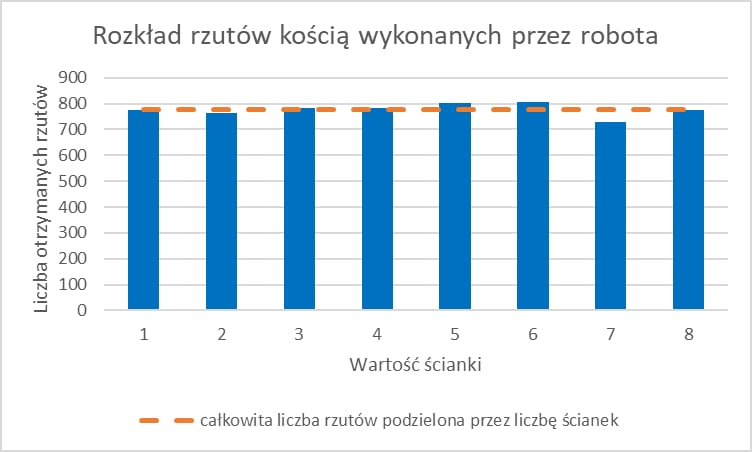
\includegraphics[width=0.75\textwidth]{chapters/06-testy/figures/robot-rzuty.jpg}
    \caption{Wykres straty modelu.}
    \label{fig:robot-wykres}
\end{figure}



\subsection{Test chi-kwadrat}
\label{chiWyniki}
Dla odczytanych wyników rzutów kością przez pierwszy model otrzymano wartość statystyki testowej chi-kwadrat równą 
246{,}079, która znacznie przekroczyła przyjętą wartość krytyczną równą \begin{math} 24{,}322 \end{math}. 
Odrzucono hipotezę \begin{math} H_0 \end{math} i przyjęto hipotezę \begin{math} H_1 \end{math}: rozkład 
prawdopodobieństwa wyników nie jest równomierny. \par
Natomiast dla drugiego modelu wartość statystyki testowej chi-kwadrat jest równa 20{,}072. Jest ona mniejsza od 
przyjętej wartości krytycznej, zatem nie ma podstaw do odrzucenia hipotezy zerowej: rozkład prawdopodobieństwa 
wyników jest równomierny. \par
Otrzymany rozkład dla obu modeli przedstawiono w tabeli \ref{chiTabela}.
\begin{table}[h]
    \centering
    \caption{Rozkład otrzymanych wyników rzutu kością}
    \label{chiTabela}
    \begin{tabular}{|c|>{\centering\arraybackslash}m{2cm}|>{\centering\arraybackslash}m{2cm}|}
        \hline
        & \multicolumn{2}{c|}{Liczba otrzymanych rzutów} \\
        \hline
        Wynik & Model 1 & Model 2 \\
        \hline
        1 & 849 & 870 \\
        \hline
        2 & 682 & 841 \\
        \hline
        3 & 952 & 838 \\
        \hline
        4 & 831 & 819 \\
        \hline
        5 & 866 & 836 \\
        \hline
        6 & 1124 & 737 \\
        \hline  
        7 & 816 & 818 \\
        \hline 
        8 & 547 & 908 \\
        \hline 
    \end{tabular} 
\end{table}


\subsection{Test monobitowy}
\label{monbitWyniki}
Dla modelu pierwszego dla otrzymanego ciągu zliczono 10694 bitów o wartości 1. Jest ona większa od oczekiwanej liczby 
jedynek. Hipotezę zerową odrzucono. Natomiast dla modelu drugiego zliczono 9805 bitów o wartości jeden. Jest to liczba
zgodna z oczekiwaną. Brak podstaw do odrzucenia hipotezy zerowej dla modelu drugiego.

\subsection{Test serii}

Wyniki testów serii dla obu modeli przedstawiono w tabeli \ref{serieTabela}. Rozkład serii w badanym ciągu odczytanym
przez pierwszy model nie jest zgodny z oczekiwanymi dla obu serii o długości 1, obu serii o długości 2, serii jedynek 
o długości 4 i serii zer o długości 6 lub więcej. Hipotezę zerową dla modelu pierwszego odrzucono.

Dla modelu drugiego rozkłady wszystkich serii są zgodne z oczekiwanymi. Brak podstaw do odrzucenia hipotezy zerowej.
\begin{table}[H]
    \centering
    \caption{Liczby wystąpień serii w ciągu}
    \label{serieTabela}
    \begin{tabular}{|c|c|c|c|c|c|} 
        \hline
        \multicolumn{2}{|c|}{} & \multicolumn{2}{c|}{Model 1} & \multicolumn{2}{c|}{Model 2} \\
        \hline
        Długość serii & Przedział & Serie zer & Serie jedynek & Serie zer & Serie jedynek \\
        \hline
        1 & 2343 - 2657 & 2717 & 2303 & 2405 & 2477 \\
        \hline
        2 & 1135 - 1365 & 1367 & 1141 & 1212 & 1250 \\
        \hline
        3 & 542 - 708 & 559 & 678 & 612 & 593 \\
        \hline
        4 & 251 - 373 & 263 & 374 & 338 & 290 \\
        \hline
        5 & 111 - 201 & 113 & 158 & 162 & 155 \\
        \hline
        6 i więcej & 111 - 201 & 82 & 177 & 194 & 159 \\
        \hline  
    \end{tabular} 
\end{table}   

\subsection{Test długich serii}
W wygenerowanym ciągu odczytanym przez model pierwszy zarówno dla zer, jak i dla jedynek, najdłuższa znaleziona seria 
zawierała 13 bitów. Jest to liczba mniejsza od maksymalnej przyjętej długości najdłuższego ciągu bitów wynoszącej 25. 
Nie ma podstaw do odrzucenia hipotezy zerowej dla modelu pierwszego. \par
Natomiast dla modelu drugiego najdłuższy nieprzerwany ciąg zer miał długość 17, a dla jedynek 16. To również są 
mniejsze wartości od maksymalnych przyjętych, zatem nie ma podstaw do odrzucenia hipotezy zerowej dla modelu drugiego.

\subsection{Test pokerowy}
\label{pokerWyniki}
Dla testu pokerowego dla modelu pierwszego otrzymano statystykę testową równą 120{,}026. Jest ona większa od oczekiwanej,
zatem odrzucono hipotezę zerową. Dla modelu drugiego statystyka testowa jest równa 28{,}794. Jest ona zgodna z wartością
oczekiwaną, zatem nie ma podstaw do odrzucenia hipotezy zerowej.
Rozkład segmentów w ciągach odczytanych przez oba modele przedstawiono w tabeli \ref{pokerTabela}.
\begin{table}[h]
    \centering
    \caption{Liczby wystąpień kombinacji bitów}
    \label{pokerTabela}
    \begin{tabular}{|c|c|c|} 
        \hline
        & \multicolumn{2}{c|}{Liczba wystąpień} \\
        \hline
        Kombinacja bitów & Model 1 & Model 2 \\
        \hline
        0000 & 197 & 361 \\
        \hline
        0001 & 249 & 310 \\
        \hline
        0010 & 277 & 347 \\
        \hline
        0011 & 312 & 317 \\
        \hline
        0100 & 279 & 246 \\
        \hline
        0101 & 309 & 280  \\
        \hline  
        0110 & 363 & 283 \\
        \hline  
        0111 & 338 & 294 \\
        \hline  
        1000 & 255 & 321 \\
        \hline  
        1001 & 355  & 276 \\
        \hline  
        1010 & 311 & 298 \\
        \hline  
        1011 & 355 & 322 \\
        \hline  
        1100 & 322 & 320 \\
        \hline  
        1101 & 335 & 297 \\
        \hline  
        1110 & 366 & 318 \\
        \hline  
        1111 & 377 & 310 \\
        \hline  
    \end{tabular} 
\end{table} 

\section{Wnioski}
Dla pierwszego modelu odrzucono hipotezę zerową dla czterech z pięciu testów. W wynikach testu statystyki 
rozkładu chi-kwadrat (sekcja \ref{chiWyniki}) można zauważyć, że liczba 6 jest odczytywana ponad dwa razy częściej niż 
liczba 8. Ma to bardzo duży wpływ na otrzymany ciąg bitów, ponieważ liczba 6 jest interpretowana jako 110, a 
liczba 8 jako 000, co można zaobserwować w wynikach pozostałych testów. Sprawia to, że jedynki pojawiają się 
częściej w ciągu niż zera. Ukazuje to już test monobitowy (sekcja \ref{chiWyniki}), gdzie liczba jedynek w ciągu jest 
większa niż oczekiwana. Podobny problem można zaobserwować w wynikach testu pokerowego (sekcja \ref{pokerWyniki}), 
gdzie segmenty zawierające trzy lub cztery bity o wartości 1 występują znacznie częściej niż segmenty zawierające 
więcej bitów o wartości 0. 

Przez wzgląd na niezadowalające wyniki modelu pierwszego, dokonano jego poprawy (sekcja \ref{sec:podsumowanie}) i
utworzono drugi model sztucznej inteligencji. Dla wszystkich przeprowadzonych testów nie było podstaw do odrzucenia
hipotezy zerowej. W przeciwieństwie do pierwszego modelu, najczęściej odczytywanym wynikiem jest 8, a najrzadziej -- 6.
Różnica w liczbie odczytów tych wyników nie jest aż tak znacząca (737 dla 6 i 908 dla 8) jak dla pierwszego modelu 
(1124 dla 6 i 547 dla 8). Częstsze wystąpienia wyniku 8 widać w teście monobitowym, gdzie zliczonych zer jest więcej
niż jedynek. Dysproporcja między nimi jest niewielka, wynosi zaledwie niecałe 400 bitów, kiedy dla pierwszego modelu
różnica wynosiła prawie 1400 bitów. Podobnie dla testu serii liczby poszczególnych serii dla zer i jedynek są dużo
bardziej zrównoważone dla drugiego modelu niż pierwszego. 

Dla testów długich serii dla obu modeli nie było podstaw do odzucenia hipotezy zerowej. Dla pierwszego z nich najdłuższe
ciągi dla obu wartości bitów miały długość 13, a dla drugiego 17 (zera) i 16 (jedynki). Ponieważ bity są generowane 
trójkami przy każdym rzucie kością, oznacza to, że dla wartości 7 (kodowanej jako 111) i 8 (kodowanej jako 000)
odczytano maksymalnie po cztery razy pod rząd dla modelu pierwszego i maksymalnie po pięć razy pod rząd dla modelu 
drugiego. 

Wyniki dla drugiego modelu są zadowalające, ponieważ nie ma dla nich przesłanek do odrzucenia żadnej z hipotez zerowych.
Jednakże w przyszłości możliwa jest implementacja lepszego modelu, który
potencjalnie mógłby otrzymywać jeszcze lepsze wyniki (rozdział \ref{ch:zakonczenie}), ponieważ wartość statystyki testowej
chi-kwadrat dla modelu drugiego jest niemal czterokrotnie większa, niż dla wartości statystyki testowej chi-kwadrat 
otrzymanej dla ręcznie oznaczone do przykładów uczących dla sieci neuronowej.
Prowadzi to do wniosku, że uzyskanie prawdziwej losowości jest możliwe, mimo deterministycznego charakteru działania maszyny.
